\chapter{Algorithmes d'optimisation}
\section{Motivation}
Il existe une grande variété d'algorithmes permettant la minimisation de la fonction de coût en plus de la descente de gradient présentée précédemment. Ce chapitre aura pour but de présenter les plus populaires d'entre eux et d'en donner les principales caractéristiques. Nous les comparerons ensuite pour retenir les solutions les plus efficaces.

\section{Descente de gradient et momentum}
\begin{equation}
W_{t+1} = W_t - \eta\frac{\partial J}{\partial W}
\end{equation} 

Les poids sont changés en fonction de la dérivée partielle de la fonction de coût par rapport à $W$. Comme vu précédemment, $\eta$ représente le learning rate. Si celui-ci est trop faible, la convergence sera lente, à l'inverse une valeur trop élevée entrainera la divergence des poids.

Cependant, le gradient de la fonction de coût change rapidement à chaque itération à cause de la diversité de chaque exemple d'apprentissage. On approchera alors le minimum par petits pas mais de façon désordonnée (en "zigzag"). En effet, si la direction moyenne obtenue sur plusieurs exemples d'apprentissage est la bonne ce n'est pas le cas si l'on ne prend en compte qu'un échantillon, celui-ci étant bruité. Cette approche consistant à calculer le gradient à chaque exemple est appelée \textit{descente de gradient stochastique}.

Pour pallier ce problème, deux solutions sont possibles. On peut moyenner le gradient sur des batchs d'exemples de longueur fixée, au risque d'avoir de la redondance et de perdre en vitesse de calcul ou en espace mémoire. On parle alors de \textit{descente de gradient par batchs}. La \textit{descente de gradient par mini-batchs} consiste à prendre les avantages des deux méthodes, en trouvant un compromis sur la taille des batchs de sorte que le temps de calcul de chaque étape ne soit pas trop long mais que les pas soient suffisamment précis pour assurer une convergence efficace.

Il est également possible d'introduire un terme de momentum. Cette opération consiste à prendre en compte l'information des itérations précédentes pour savoir dans quelle direction il est préférable de progresser. En introduisant à cet effet un nouvel hyperparamètre $\mu$, on obtient alors les équations de mise à jour des poids ci-dessous.

\begin{equation}
\begin{aligned}
v_{t+1} = \mu v_t - \eta\frac{\partial J}{\partial W}\\
W_{t+1} = W_t + v_t
\end{aligned}
\end{equation} 

La trajectoire est alors plus lisse et la convergence plus efficace.

\section{Algorithmes à learning rate adaptatif}
\subsection{Adagrad}

L'objectif de cet algorithme est de ne plus avoir de learning rate constant mais d'adapter celui-ci en fonction de la valeur du gradient aux étapes précédentes. Cela se traduit dans l'équation de mise à jour des poids par une division par un terme $g_t$, somme des carrés des gradients des itérations précédentes.
On obtient finalement les équations suivantes :

\begin{equation}
\begin{aligned}
g_{t+1} = g_t + (\frac{\partial J}{\partial W})^2 \\
W_{t+1} = W_t - \dfrac{\eta\frac{\partial J}{\partial W}}{\sqrt{g_{t+1}} + \epsilon}
\end{aligned}
\end{equation} 

Le terme $\epsilon$ sert à initialiser l'algorithme et permet de s'assurer que le dénominateur ne sera jamais nul. On observe que si la norme du gradient est grande, le learning rate sera faible et vice versa. 
On n'a donc plus besoin de changer le learning rate manuellement, celui-ci est simplement fixé au départ puis adapté automatiquement. Cependant, comme le terme au dénominateur va augmenter au fur et à mesure, les termes $g_t$ étant tous positifs, le learning rate aura tendance à devenir de plus en plus faible jusqu'à devenir infinitésimal. Les algorithmes suivants permettront de résoudre ce problème.

\subsection{RMSProp}

La principale différence avec Adagrad est que le terme $g_t$ est calculé grâce à une moyenne mobile exponentielle : on utilise alors une pondération des termes qui décroît exponentiellement, ce qui donne plus d'importance aux valeurs récentes du gradient sans pour autant supprimer complètement les anciennes contributions. 

\begin{equation} 
\begin{aligned}
g_{t+1} = \gamma g_t + (1-\gamma)(\frac{\partial J}{\partial W})^2 \\
W_{t+1} = W_t - \dfrac{\eta\frac{\partial J}{\partial W}}{\sqrt{g_{t+1}} + \epsilon}
\end{aligned}
\end{equation} 

En raison du terme quadratique présent lors du calcul de $g_t$, ce dernier est appelé \textbf{moment d'ordre 2} de $\frac{\partial J}{\partial W}$. On trouve dans certaines implémentations l'ajout d'un moment d'ordre 1, qui se définit de façon très similaire par :
\begin{equation} 
m_{t+1} = \gamma m_t + (1-\gamma)(\frac{\partial J}{\partial W})
\end{equation} 

Il est même possible de rajouter un terme de momentum comme pour la descente du gradient stochastique, les équations de mise à jour finales sont alors :

\begin{equation} 
\begin{aligned}
v_{t+1} = \mu v_t - \dfrac{\eta \frac{\partial J}{\partial W}}{\sqrt{g_{t+1}-m^2_{t+1}+\epsilon}}\\
W_{t+1} = W_t + v_{t+1}
\end{aligned}
\end{equation} 

\subsection{Adadelta}

Cet algorithme utilise également une moyenne mobile exponentielle pour le calcul de $g_t$, moment d'ordre 2 du gradient. Cependant, au lieu d'utiliser un hyperparamètre $\eta$ fixe comme précédemment, il introduit à la place $x_t$, moment d'ordre 2 de $v_t$.

\begin{equation} 
\begin{aligned}
g_{t+1} = \gamma g_t + (1-\gamma) (\frac{\partial J}{\partial W})^2 \\
x_{t+1} = \gamma x_t + (1-\gamma)v^2_{t+1}
\end{aligned}
\end{equation}


Les équations finales sont alors, si l'on se limite aux moments d'ordre 2 et sans momentum :

\begin{equation}
\begin{aligned}
v_{t+1} = - \dfrac{\sqrt{x_t + \epsilon}\frac{\partial J}{\partial W}}{\sqrt{g_{t+1}+\epsilon}}\\
W_{t+1} = W_t + v_{t+1}
\end{aligned}
\end{equation}
 
\subsection{Adam}

Le dernier algorithme présenté consiste à reprendre les moments d'ordre 1 et 2 du gradient, $m_t$ et $g_t$, mais en les faisant cette fois-ci décroître dans le temps à l'aide de coefficients $\gamma_1$ et $\gamma_2$ $\in$ [0,1[

\begin{equation}
\begin{aligned}
\hat{m}_{t+1}=\dfrac{m_{t+1}}{1-\gamma^{t+1}_1}
\hat{g}_{t+1}=\dfrac{g_{t+1}}{1-\gamma^{t+1}_2}
\end{aligned}
\end{equation}

Cela aura donc pour effet de réduire la taille des pas à l'approche du minimum et donc d'assurer une bonne convergence grâce à une adaptation efficace du learning rate. On obtient finalement l'équation de mise à jour des poids suivante :

\begin{equation}
\begin{aligned}
W_{t+1}=W_t - \dfrac{\alpha\hat{m}_{t+1}}{\sqrt{\hat{g}_{t+1}}+\epsilon}
\end{aligned}
\end{equation}

\section{Comparaison des algorithmes}

Nous avons eu l'occasion d'implémenter ces différents algorithmes et de les appliquer aux problèmes précédents. S'il n'y a pas à l'heure actuelle de consensus sur le meilleur d'entre eux, certaines solutions se sont révélées être bien plus efficaces que d'autres dans notre cas.

\subsection{Application à l'apprentissage du XOR}

\begin{figure}[!h]
\begin{center}
	{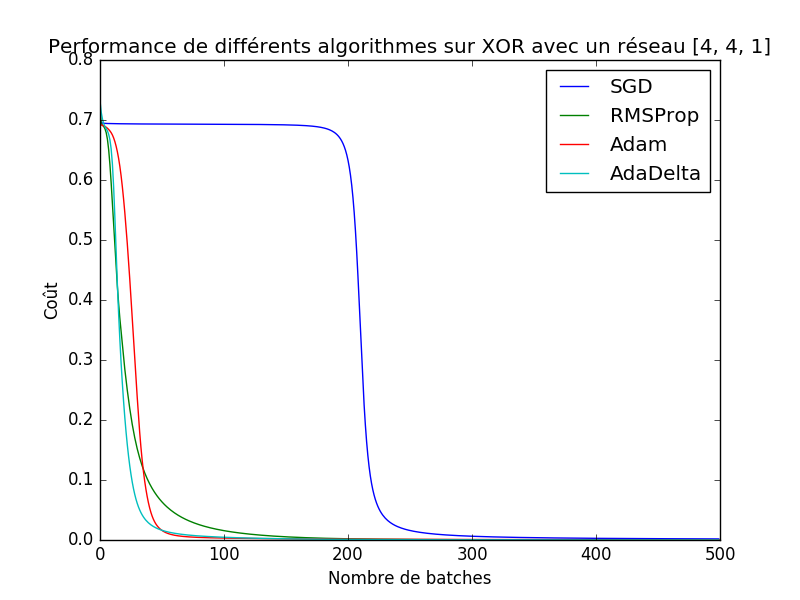
\includegraphics[scale=0.4]{images/chapter8/xor_comparison_algo.png}\label{Algorithmes}}
  \caption{Comparaison des fonctions de coût pour les différents algorithmes appliqués au XOR}
\end{center}
\end{figure}

On observe que les fonctions de coût pour les algorithmes à learning rate adaptatif ont des profils très similaires et ne présentent pas le pallier observé pour la descente de gradient stochastique. L'apprentissage est presque 4 fois plus rapide pour des temps de calcul du même ordre de grandeur, ce sont donc de meilleures implémentations en tout point pour ce type de problème.

\subsection{Application à l'apprentissage des oeuvres de Shakespeare}

\begin{figure}[!h]
\begin{center}
	{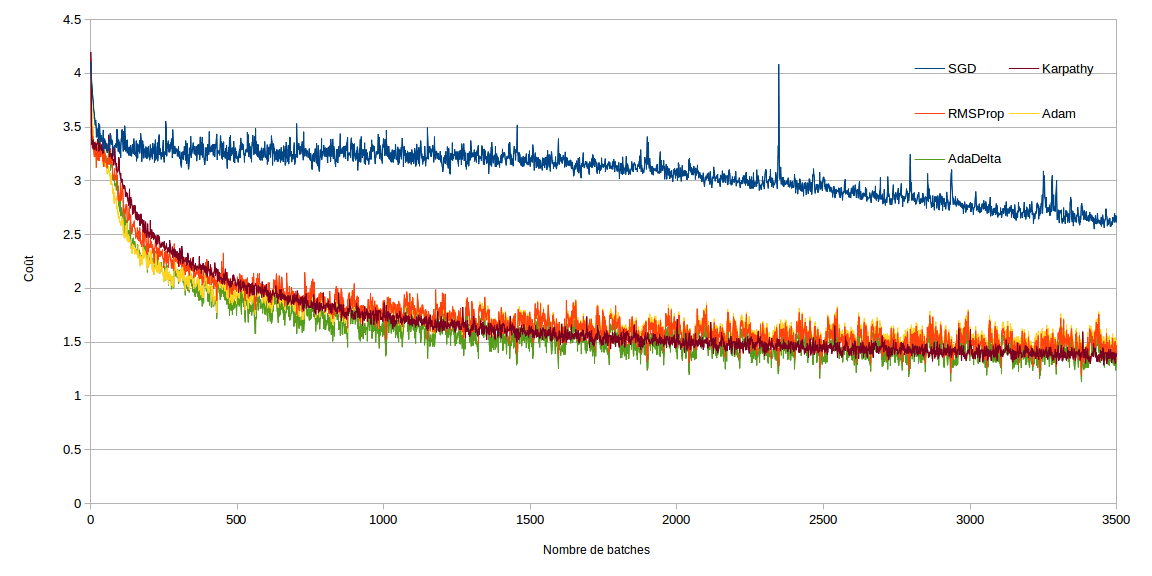
\includegraphics[scale=0.4]{images/chapter8/comparison.png}\label{Algorithmes}}
  \caption{Comparaison des fonctions de coût pour les différents algorithmes appliqués à Shakespeare aux côtés de l'implémentation d'Andrej Karpathy}
\end{center}
\end{figure}

La différence entre la descente de gradient stochastique et les autres algorithmes est encore plus flagrante dans ce cas : la convergence est bien plus rapide, nécessitant bien moins d'exemples d'apprentissage. Nous avons donc par la suite totalement délaissé la descente de gradient classique au profit de RMSProp ou Adam, beaucoup plus performants.

\section {Conclusion}
Si la descente du gradient stochastique est l'algorithme le plus répandu dans la littérature, il existe de nombreuses autres méthodes d'optimisation pour la minimisation de la fonction de coût. Nous avons présenté les plus populaires d'entre elles dans ce chapitre et avons réalisé qu'elles permettaient d'avoir de bien meilleures performances pour les applications que nous avons considérées. 

Il existe également une autre famille d'algorithmes du second ordre que nous n'avons pas eu le temps d'implémenter (méthode de Newton, BFGS, conjugate gradient...). Cependant, si nous avons trouvé des implémentations des algorithmes de ce chapitre dans des projets disponibles sur Internet, ce n'est pas le cas des méthodes du second ordre. Il est donc possible que ces dernières soient moins efficaces, que ce soit au niveau du temps de calcul ou de l'espace mémoire, bien que cela reste à vérifier.